\documentclass[a4paper, notitlepage, 10pt]{article}
\usepackage{geometry}
% WSC 2015 configs
\fontfamily{times}
\geometry{verbose,tmargin=30mm,bmargin=25mm,lmargin=25mm,rmargin=25mm}
\pagestyle{empty}
% end configs
\usepackage{setspace,relsize}               
\usepackage{moreverb}                        
\usepackage{url}
\usepackage{hyperref}
\hypersetup{colorlinks=true,citecolor=blue}
\usepackage{amsmath}
\usepackage{mathtools} 
\usepackage{amsthm}
\usepackage{amssymb}
\usepackage{indentfirst}
\usepackage{todonotes}
\usepackage[authoryear,round]{natbib}
\bibliographystyle{apalike}
\usepackage[pdftex]{lscape}
\usepackage[utf8]{inputenc}
% Title Page
\title{\vspace{-9ex}\centering \bf On the choice of the weights for the logarithmic pooling of probability distributions}
\author{
Luiz Max F. de Carvalho$^{a,b,c}$, Daniel A. M. Villela$^a$, Flavio Coelho$^c$ \& Leonardo S. Bastos$^a$ \\
a -- Program for Scientific Computing (PROCC), Oswaldo Cruz Foundation. \\
b -- Institute of Evolutionary Biology, University of Edinburgh.\\
c -- School of Applied Mathematics, Getulio Vargas Foundation (FGV).
}
\DeclareMathOperator*{\argmin}{arg\,min}
\DeclareMathOperator*{\argmax}{arg\,max}
\newtheorem{theo}{Theorem}[]
\newtheorem{proposition}{Proposition}[]
\newtheorem{remark}{Remark}[]
\setcounter{theo}{0} % assign desired value to theorem counter
\begin{document}
\maketitle

\begin{abstract}
Combining different prior distributions is an important issue in decision theory and Bayesian inference.
Logarithmic pooling is a popular method to aggregate expert opinions by using a set of weights that reflect the reliability of each information source.
The resulting pooled distribution however heavily depends set of weights given to each opinion/prior.
In this paper we explore three approaches to assigning weights to opinions.
Two methods are stated in terms of optimisation problems and a third one uses a hierarchical prior that accounts for uncertainty on the weights. 
We explore several examples of interest, such as proportion and rate estimation and combining Normal distributions.
Our findings...

Key-words: logarithmic pooling; expert opinion; maximum entropy; Kullback-Leibler divergence; Dirichlet prior. 
\end{abstract}

\section*{Background}

Combining probability distributions is a topic of general interest, both in the statistical~\citep{west1984, genest1986A, genest1986B} and decision theory literatures~\citep{genest1984}.
On the theoretical front, studying opinion pooling operators may give important insights on consensus belief formation and group decision making~\citep{genest1986B}.
Among the various opinion pooling operators proposed in the literature, logarithmic pooling has enjoyed much popularity, mainly due to its many desirable properties such as relative propensity consistency (RPC) and external Bayesianity (EB)~\citep{genest1986A}. 
In a practical setting, logarithmic pooling finds use in a range of fields, from infectious disease modelling~\citep{Coelho2009} and wildlife conservation~\citep{poole2000} to engineering~\citep{lind1988, savchuk1994}.

A common situation of interest is that of combining expert opinions, represented as proper probability distributions, about a quantity of interest $\theta \in \mathbf{\Theta} \subseteq \mathbb{R}^n$.
To combine these opinions using logarithmic pooling requires assigning weights to each of the experts.
These weights represent the reliability of each opinion~\citep{genest1984}.
This requirement naturally leads to the question of how to choose the weights in a meaningful fashion, according to some well-accepted optimality criterion.
There are a few proposals in the literature that build methods using different approaches.
One proposal is to maximise the entropy the pooled distribution~\citep{myung1996}, whereas another one is to minimise Kullback-Leibler (KL) divergence between the pooled distribution and the individual opinions~\citep{abbas2009} or between the pooled (prior) distribution and the posterior distribution~\citep{rufo2012A,rufo2012B}.

These approaches, while moving away from the problem of arbitrarily assigning the weights, arrive at single point solutions, similar to point estimates in Statistical theory.
Albeit acknowledging that these approaches have merit, we argue that in many settings, where one has substantial prior information on the relative reliabilities of the information sources (experts), it would be desirable to incorporate this information into the pooling procedure while accommodating uncertainty about the weights~\citep{poole2000}.
Moreover, assigning a probability distribution to the weights permits us to obtain a posterior distribution using a Bayesian procedure, which in turn enables us to learn about these weights.
Therefore, it makes possible to sequentially update knowledge about the reliability of each expert/source in the face of new data.

In this paper we explore previous approaches for deriving the weights for logarithmic pooling, namely by maximising the entropy of the resulting distribution and minimising the KL divergence between the pooled distribution and each individual distribution.
Additionally, we propose a hierarchical prior approach in which we place a distribution on the weights.
We present an example on proportion estimation by combining Beta priors.
[EXEMPLO]

\section*{Properties of the logarithmic pooling operator}

In what follows, we introduce the necessary theory and motivate the use of the logarithmic pooling operator by presenting some of its desirable properties.

Let $\mathbf{F}_{\theta} := \{f_0(\theta), f_1(\theta), f_2(\theta), \ldots, f_K(\theta)\}$ be a set of prior distributions representing the opinions of $K+1$ experts and let $\boldsymbol\alpha :=\{\alpha_0, \alpha_1, \alpha_2, \ldots, \alpha_K \}$ be the vector of weights, such that $\alpha_i > 0\: \forall i$ and $\sum_{i=0}^K \alpha_i = 1$.
Then the log-pooled prior is
\begin{equation}
\label{eq:logpool}
 \pi(\theta) := t(\boldsymbol\alpha) \prod_{i=0}^K f_i(\theta)^{\alpha_i},
\end{equation}
where $t(\boldsymbol\alpha) = \int_{\boldsymbol\Theta}\prod_{i=0}^K f_i(\theta)^{\alpha_i}d\theta$.

Logarithmic pooling will only yield proper probability distributions if it is possible to normalise the expression in (\ref{eq:logpool}).
This condition is usually assumed implicitly, without proof.
\citet{poole2000} provide a proof for the case of two densities (see Theorem 1 therein), which we extend for the case of a finite number of densities.
\begin{theo}
\label{thm:normalisation}
\textbf{Normalisation}. 
Let $A$ be the $(K+1)$-dimensional open simplex on $[0,1]$.
For all $\boldsymbol\alpha \in A$ there exists a constant $t(\boldsymbol\alpha)$ such that $\int_{\boldsymbol\Theta}\pi(\theta)d\theta = 1$.
\end{theo}

This result ensures any (finite) number of proper distributions can be combined using the logarithmic pooling operator to yield a normalisable density.

Another interesting property of the logarithmic pooling operator is the fact that combining log-concave densities will produce a log-concave pooled distribution.
\begin{remark}
\label{rmk:concavity}
\textbf{Log-concavity}. 
 Let $\mathbf{F}_{\theta}$ be a set of log-concave distributions, i.e., each $f_i$ can be represented as
 \begin{equation}
  \label{eq:logconcavity}
  f_i(\theta) \propto e^{\psi_i(\theta)},
 \end{equation}
where $\psi_i(\cdot)$ is a concave function.
Then $\pi(\theta)$ is also log-concave.
\end{remark}

Log-concavity of the pooled prior may be important to consider in order to guarantee unimodality and certain conditions on tail behaviour.

\subsection*{Exponential family}

Suppose we are interested in a random variable, $Y$, from a exponential family with parameter $\theta$ and probability density function is given by
\begin{equation}
\label{eq:exponentialfamily}
f(y|\theta) = h(y) e^{\theta y - \psi(\theta)}.
\end{equation}

Let $\mathbf{F}_{y}$ be a set of distributions on $y$ of the form in~(\ref{eq:exponentialfamily}), $f_i(y|\theta_i)$, $ i = 0, 1, \ldots, K$. 
The combined (log-pooled) distribution also belongs to the exponential family:

\begin{equation}
\label{eq:pooldistEF}
\pi(y|\boldsymbol\alpha) = t(\boldsymbol\alpha) h^\ast (y) e^{\theta^\ast y - \psi^\ast (\tilde{\theta})}.
\end{equation}
where $h^\ast (y) = \prod_{i = 0}^K h_i(y)^{\alpha_i}$,  $\theta^\ast = \sum_{i = 0}^K \alpha_i \theta_i$ and $\psi^\ast (\tilde{\theta}) = \sum_{i = 0}^K \alpha_i \psi_i(\theta_i)$.

The entropy function of the log-pooled distribution is
\begin{equation}
\label{eq:entropydistEF}
H_\pi(y) =  -\log t(\boldsymbol\alpha) + \psi^\ast (\tilde{\theta}) - \mathbb{E}_\pi[\log h^\ast (y)] - \theta^\ast\mathbb{E}_\pi[Y] \: ,
\end{equation}
and the Kullback-Leibler divergence between each distribution in $\mathbf{F}_{y}$ and $\pi(y|\boldsymbol\alpha)$ can be written as:
\begin{equation}
\label{eq:KLdistEF}
KL(f_i || \pi)  =  -\psi_i(\theta_i) +   \psi^\ast (\tilde{\theta}) +  \mathbb{E}_\pi[\log h_i(y)] - \mathbb{E}_\pi[\log h^\ast (y)] \: .
\end{equation}

These expressions allow for easy computation of information measures for a broad class of distributions, which will be useful in the remainder of this paper.

\subsubsection*{Conjugate priors}

A conjugate prior family for $f(y|\theta)$ is the following
\begin{equation}
\label{eq:priorEF}
g(\theta | a, b) = K(a,b) e^{\theta a - b \psi(\theta)} \: ,
\end{equation}
where $K(a,b)$ is a normalising constant.
Here, we employ the definition and notation for exponential family and its conjugate prior family from \citet[chapter 3]{robert2001bayesian}.
Similar to the above, let $\mathbf{G}_{\theta}$ be a set of conjugate prior distributions representing the opinions of $K+1$ experts, and $g_i(\theta) = g(\theta | a_i, b_i)$ from equation (\ref{eq:priorEF}).

The log-pooled prior is also a conjugate prior for $f(y|\theta)$ with hyperparameters given by an weighted mean of the experts hyperparameters, i.e.
\begin{equation}
\label{eq:poolpriorEF}
\pi(\theta|\boldsymbol\alpha) = g(\theta | a^*, b^*) \: ,
\end{equation}
where $a^* = \sum_{i} \alpha_i a_i$ and $b^* = \sum_{i} \alpha_i b_i$.
Note that the posterior distribution of $\theta$ is given by $\pi(\theta | y) = g(\theta | a^* + y, b^* + 1)$.

The entropy function of the log-pooled prior is given by
\begin{equation}
\label{eq:entropypriorEF}
H_\pi(\theta) = - \log (K(a^*, b^*)) + a^*  E[\theta]-  b^*  E[\psi(\theta)] \: .
\end{equation}

And the Kullback-Leibler divergence, $KL(f_i || \pi)$, is the following
\begin{equation}
\label{eq:KLpriorEF}
KL(g_i || \pi) = \log( K(a_i,b_i)) - \log(K(a^*,b^*)) + (a_i - a^*) E[\theta] - (b_i - b^*) E[\psi(\theta)] \: .
\end{equation}

\section*{Induce-then-pool or pool-then-induce?}

Let $\theta \in \Theta \subseteq \mathbb{R}^p$ and $y \in \mathcal{Y} \subseteq \mathbb{R}^p$. 
Define the model (transformation) as $M \,:\, \Theta \to \mathcal{Y}$. 
This paper concerns the setting where a set $\mathbf{F_\theta}$ of distributions on $\theta$ is available but one is interested in obtaining a pooled distribution on $y$.
There are two ways of obtaining a pooled distribution $\pi(y)$: (a) combine the distributions in $\mathbf{F_\theta}$ and then apply $M(\cdot)$ to the resulting distribution to get the \underline{induced} distribution on $y$ (``pool-then-induce'') or; (b) apply  $M(\cdot)$ to each component of $\mathbf{F_\theta}$ and combine the resulting induced distributions using the logarithmic pooling operator (``induce-then-pool''). 
First we note that under some conditions on the transformation $M(\cdot)$, the order in which one performs the pooling and transforming operations does not matter.
%% "Stolen" from http://math.stackexchange.com/questions/732960/inverse-of-a-multivariable-function
Consider $M(\theta) = y$ and suppose $M(\cdot)$ is invertible, i.e., there exists $M^{-1}: \: \mathcal{Y} \to \Theta$ such that,
\[A_0:\quad M(M^{-1}(v)) = v,\: v \in \mathcal{Y}\: \text{and}\: M^{-1}(M(t)) = t, \: t \in \Theta \]
and $J := det \left[ \frac{\partial M^{-1}}{\partial y_1}, \frac{\partial M^{-1}}{\partial y_2}, \ldots, \frac{\partial M^{-1}}{\partial y_p}\right]$ is the Jacobian.

With some abuse of notation, define
  \begin{align}
  \label{eq:transfF}
  \mathbf{F^{-1}_y} &:= \{h_1(y), \, h_2(y), \ldots, \, h_K(y) \} \\
  h_i(y) & = f_i(M^{-1}(y))|J|\nonumber
  \end{align}
where $|J|$ is the absolute value of $J$.
\begin{remark}
\label{rmk:invariance}
Define $\pi_{\theta}(\theta | \boldsymbol\alpha) =  \mathcal{LP}(\mathbf{F_\theta}, \boldsymbol\alpha)$ and $\pi_{y}(y |\boldsymbol\alpha) = \pi_{\theta}(M^{-1}(y))|J|$.
Similarly, define $\pi^{\prime}_{y}(y|\boldsymbol\alpha) = \mathcal{LP}(\mathbf{F^{-1}_y}, \boldsymbol\alpha)$.
If $A_0$ is satisfied, then $\pi_{y}(y |\boldsymbol\alpha) = \pi^{\prime}_{y}(y|\boldsymbol\alpha)$, i.e., the order in which one combines and transforms the distributions does not matter.
\end{remark}
\begin{proof}
To see that Remark~\ref{rmk:invariance} holds, we only need a straightforward calculation from the definition of the logarithmic pooling operator in~(\ref{eq:logpool}):
\[\pi_{y}(y |\boldsymbol\alpha) \propto \prod_{i=0}^K f_i(M^{-1}(y))^{w_i}|J| \]
whereas
\begin{align*}
 \pi^{\prime}_{y}(y|\boldsymbol\alpha) &\propto  \prod_{i=0}^K \left[ f_i(M^{-1}(y))|J| \right] ^{w_i} = \prod_{i=0}^K f_i(M^{-1}(y))^{w_i} \prod_{i=0}^K|J|^{w_i}\\
 &\propto  \prod_{i=0}^K f_i(M^{-1}(y))^{w_i}|J|, %TODO: maybe = instead of \propto ?
\end{align*}
as claimed.
%% LM: if this embarassingly simple ``proof'' does not convince you, take a look at https://github.com/maxbiostat/R0_uncertainty/blob/master/code/invertible_model_equivalence.r
This is very similar in nature to the ``external Bayesianity'' property of the logarithmic pooling operator, by which one can either pool the prior distributions and then combine the resulting distribution with the likelihood or combine each prior with the likelihood separately and then pool the resulting posteriors to obtain the same posterior distribution.
%% TODO: if we can show that combining the prior with the likelihood is an invertible transform, then this result is a generalisation of EB. But we first need to see the degree of generality EB was actually proven in the original paper.
\end{proof}

\textbf{\large Can we prove the reverse (Equivalence$\to$Invertibility) ?}

Here go my two cents.
Suppose $M(\cdot)$ is not invertible on the whole of $\mathcal{Y}$, but instead is \textbf{piece-wise invertible}.
Let $\mathcal{Y}_1, \mathcal{Y}_2, \ldots, \mathcal{Y}_T$ be a  partition of $\mathcal{Y}$, i.e., $\mathcal{Y}_i\cap\mathcal{Y}_j = \emptyset,\: \forall i\neq j \in \{1, 2, \ldots, T\}$ and $\bigcup_{t = 1}^T\mathcal{Y}_t = \mathcal{Y}$.
Then define the inverse functions $M_{t}^{-1}(y)\,:\, \mathcal{Y}_t \to \Theta, \: t \in \{1, 2, \ldots, T\}$.
Last, let $J_t$ be the Jacobian of $M_{t}^{-1}(\cdot)$.
Then we are prepared to write:
\begin{align}
\label{eq:piecewiseTransf}
\pi_{y}(y |\boldsymbol\alpha) &\propto \sum_{t = 1}^T\left(\prod_{i=0}^K f_i(M_t^{-1}(y))^{w_i}\right)|J_t|, \quad \text{and}\\
\pi^{\prime}_{y}(y|\boldsymbol\alpha) &\propto \prod_{i=0}^K\left[\sum_{t = 1}^T f_i(M_t^{-1}(y))|J_t|\right]^{w_i}
\end{align}
which, I claim, will only be equal if $T = 1$, that is,  if $M(\cdot)$ is invertible in the usual sense.


We now move on to study three approaches to assign weights.
The first two approaches are based on optimality criteria and a third method is based on assigning a Dirichlet hyperprior on the weights.
\section*{Methods}
\subsection*{Choosing the weights based on optimality criteria}
\subsubsection*{Maximum entropy}

In a context of near complete uncertainty about the relative reliabilities of the experts (information sources) it may be desirable to combine the prior distributions such that $\pi(\theta)$ is maximally uninformative. %% LM: this can be highly problematic...
Such approach would ensure that, given the constraints imposed by $\mathbf{F}_{\theta}$, the pooled distribution is the one which best represents the current state of knowledge~\citep{jaynes1957,savchuk1994}.
In order to choose $\boldsymbol\alpha$ so as to maximise prior 
diffuseness, one can maximise the entropy of the log-pooled prior:
\begin{equation}
\label{eq:entropypiA}
H_{\pi}(\theta) = E_{\pi}\left[-\ln\pi(\theta) \right] =-\int_{\boldsymbol\Theta}\pi(\theta)\ln\pi(\theta)d\theta 
\end{equation}

In some cases it may be useful to express $H_{\pi}(\theta)$ as
\begin{equation}
\label{eq:entropypiB}
 H_{\pi}(\theta; \boldsymbol\alpha) = \sum_{i=0}^{K} \alpha_i E_{\pi}[ - \ln f_i(\theta)] - \ln t(\boldsymbol\alpha)
\end{equation}
Formally, we want to find $\hat{\boldsymbol\alpha}$ such that
\begin{equation}
\label{eq:argmaxEnt}
 \hat{\boldsymbol\alpha}:= \argmax H_{\pi}(\theta; \boldsymbol\alpha)  
\end{equation}

This approach, however, does not result in a convex optimisation problem, therefore one is not guaranteed to find a unique solution. 
See Proposition~\ref{remark:uniqueness}, below, for intuition as to why.

\subsubsection*{Minimising Kullback-Leibler divergence}

One could also want to choose the pooling weights so as to minimise the total Kullback-Leibler divergence between each proposed distribution and the pooled distribution.
Let $d_i = \text{KL}(f_i || \pi)$ and let $L(\boldsymbol\alpha)$ be a loss function such that
\begin{align}
L(\boldsymbol\alpha) &= \sum_{i=0}^Kd_i \\
\label{eq:KLexpanded}
     &= -K\ln t(\boldsymbol\alpha) + \sum_{i=0}^K\sum_{j\neq i}^K\alpha_j\text{KL}(f_i||f_j) \\
     \label{eq:argminKL}
     \hat{\boldsymbol\alpha}:=& \:\argmin L(\boldsymbol\alpha)   
\end{align}

\begin{remark}
\label{remark:uniqueness}
\textbf{Uniqueness}~\citep{rufo2012A}.
 The distribution obtained following~(\ref{eq:argminKL}) is unique, i.e., there is only one aggregated prior $\pi(\theta)$ that minimizes $L(\boldsymbol\alpha)$.
\end{remark}
One can get some intuition into the proof  of this claim by noting that minimising~(\ref{eq:KLexpanded}) is equivalent to maximising $\ln t(\boldsymbol\alpha) = \ln\int_{\boldsymbol\Theta}\prod_{i=0}^{K}f_i(\theta)^{\alpha_i}d\theta$. 
\cite{rufo2012A} show that $t(\boldsymbol\alpha)$ is concave, therefore the problem in~(\ref{eq:argminKL}) has a unique solution.
By contrast, the problem in~(\ref{eq:argmaxEnt}) requires to minimise $\ln t(\boldsymbol\alpha)$ hence lacking a sufficient condition for the existence of a unique solution.

\subsubsection*{Minimising Kullback-Leibler divergence in transformed space}

One might argue that procedure (b) makes little sense, given that the set of opinions $\mathbf{F}_{\theta}$ concerns only $\theta$, i.e, it was not necessarily constructed taking the transformation $M(\cdot)$ into account.
An example is a situation where experts are asked to provide distributions on the probability $p$ of a particular event.
In general, elicitation for $f_i(p)$ will not take into account the induced distribution on the log-odds, $M(p) = \log p/(1-p)$.
%% LM: we can change this dull example to something more involved.
Nevertheless, the decision-maker may wish to assign the weights $\boldsymbol\alpha$ in a way that takes $M(\cdot)$ into account, e.g., by giving lower weights to experts whose distributions on the log-odds scale are unreasonable.

This decision process can be made more precise.
In a similar spirit to the discussed above, one can construct $\boldsymbol\alpha$ so as to minimise the Kullback-Leibler divergence between each distribution in $\mathbf{F^{-1}_y}$ and a transformation of the distribution obtained by procedure (a), $\pi_{y}(y | \boldsymbol\alpha) = \pi_{\theta}( M^{-1}(y)| \boldsymbol\alpha)|J|$.
Let $d_i = \text{KL}( h_i(y) || \pi_{y}(y | \boldsymbol\alpha))$.
We then aim at solving the problem
\begin{align}
L(\boldsymbol\alpha) &= \sum_{i=0}^Kd_i \\
     \hat{\boldsymbol\alpha}:=& \:\argmin L(\boldsymbol\alpha)  \nonumber
\end{align}

This procedure therefore choses weights for each expert by how coherent the prior provided by each expert is with the pool-then-induce -- procedure (a) -- prior in the transformed space induced by $M(\cdot)$.

\subsection*{Specifying a prior distribution for $\boldsymbol\alpha$}

In this section we propose a hierarchical prior for $\theta$ conditional on $\boldsymbol\alpha$ in order to incorporate uncertainty on the weights.
A natural choice for a prior distribution for $\boldsymbol\alpha$ is the $(K+1)-$dimensional Dirichlet distribution.
The conditional distribution $\pi(\theta|\boldsymbol\alpha)$ is of the form in~(\ref{eq:logpool}) and the prior density for $\boldsymbol\alpha$ is 
\begin{equation}
 \label{eq:generalcondprior}
 \pi(\boldsymbol\alpha) = \frac{1}{\mathcal{B}(\boldsymbol X)}\prod_{i=0}^K \alpha_i^{x_i-1}
\end{equation}
where $\boldsymbol X = \{ x_0, x_1, \ldots, x_K\}$ is the vector of hyperparameters for the Dirichlet prior and $\mathcal{B}(X)$ is the multinomial beta function.
The marginal prior for $\theta$ is then
\begin{align}
 \label{eq:marginalhierprior}
 \pi(\theta) &= \int_{A}\pi(\theta|\boldsymbol\alpha)\pi(\boldsymbol\alpha)d\boldsymbol\alpha \\
             &= \frac{1}{\mathcal{B}(\boldsymbol X)}\int_{A}t(\boldsymbol\alpha)\prod_{i=0}^K f_i(\theta)^{\alpha_i}\alpha_i^{x_i-1}d\boldsymbol\alpha 
\end{align}

\section*{Applications}
\label{sec:apps}

\subsection*{Binomial probabilities}
\label{sec:beta}
We now turn our attention to combining expert opinions about probabilities and proportions.
In this setting we are interested in the random variable $Y | \theta \sim Bernoulli(\theta)$.
Assume that we want to obtain a combined prior for a proportion $\theta$.
A common choice for $\mathbf{F}(\theta)$ is the Beta family of distributions:
$$f_i(\theta;a_i, b_i) = \frac{\Gamma(a_i + b_i)}{\Gamma(a_i b_i)} \theta^{a_i-1}(1-\theta)^{b_i-1}$$
The log-pooled prior is then
\begin{align}
\pi(\theta)&= t(\boldsymbol\alpha)\prod_{i=0}^{K}f_i(\theta;a_i,b_i)^{\alpha_i}\\
&\propto \prod_{i=0}^{K} \left(\theta^{a_i-1}(1-\theta)^{b_i-1} \right)^{\alpha_i}\\
\label{eq:betabern}
&\propto \theta^{a^*-1}(1-\theta)^{b^*-1}
\end{align}
with $a^* =\sum_{i=0}^{K}\alpha_ia_i$ and $b^* = \sum_{i=0}^{K}\alpha_ib_i$.
Note that (\ref{eq:betabern}) is the kernel of a Beta distribution with parameters $a^*$ and $b^*$, thus 
\begin{equation}
 \label{eq:entropybeta}
 H_{\pi}(\theta) = \ln B(a^*,b^*) - (a^*-1)\psi(a^*) - (b^*-1)\psi(b^*) + (a^*+b^* -2)\psi(a^*+b^*)
\end{equation}

For the beta family of distributions, the KL divergence between $f_i(\theta)$ and $\pi(\theta)$ is
\begin{equation}
\begin{split}
 \label{eq:KLbeta}
 d_i = KL(f_i||\pi) = \ln\left(\frac{\mathcal{B}(a^*, b^*)}{\mathcal{B}(a_i, 
b_i)}\right) &+ (a_i-a^*)\psi(a_i)+ (b_i-b^*)\psi(b_i) \\
 &+ (a^*-a_i + b^* - b_i)\psi(a_i+b_i)
\end{split}
 \end{equation}

The marginal prior for $\theta$ is
\begin{equation}
\label{eq:marginalbeta}
\pi(\theta) = \frac{1}{\mathcal{B}(X)}\int_{A} \frac{1}{\mathcal{B}(a^*, b^*)} \theta^{a^* -1}(1-\theta)^{b^* -1}\alpha_i^{x_i-1}d\boldsymbol\alpha 
\end{equation}
which can also be efficiently approximated through Monte Carlo sampling.
We provide a simple implementation using the Stan~\citep{stan2014} probabilistic programming language at~\url{https://github.com/maxbiostat/opinion_pooling}.
R code for the methods, figures and tables presented in this paper can also be found at the above link.

Here we analyse an example proposed by~\cite{savchuk1994} (also discussed in~\cite{rufo2012B}) in which four experts are required supply prior information about the survival probability of a certain unit for which there have been $y = 9$ successes out of $n = 10$ trials.
The experts express their opinion as prior means for the survival probability, which~\cite{savchuk1994} then use to construct prior distributions with maximum variance given the restriction on the means.
From the vector of prior means $\mathbf{m} = \{ m_0 = 0.95, m_1 = 0.80, m_2 = 0.90, m_3 = 0.70 \}$, the authors obtain the parameters of the beta distributions for each expert,  $\mathbf{a} = \{ a_0 = 18.10, a_1 = 3.44 , a_2 = 8.32, a_3 = 1.98 \}$ and  $\mathbf{b} = \{ b_0 = 0.955 , b_1 = 0.860, b_2 = 0.924, b_3 = 0.848\}$.
The resulting prior densities are show in the top panel of Figure~\ref{fig:priors_posteriors_beta}.
To complete the analysis, we place a diffuse $Dirichlet(\boldsymbol\alpha | \boldsymbol X)$ prior on $\boldsymbol\alpha$ with $X_i = 1/4 \: \forall i$.
Finally, we propose to compare the prior distributions representing the experts' opinions as well as the combined distributions obtained by the different approaches using the integrated (marginal) likelihood (\cite{raftery2007}, eq. 9), $l(y) = \int_{0}^{1}f(y|\theta)\pi(\theta)d\theta$.
The marginal likelihood for the $i-th$ expert and $J$ observations of the form $\{ y_j, n_j\}$ is:
\begin{align}
  \label{eq:marglike}
l_i(y_j) &= \int_{0}^{1}\mathcal{L}(\theta|y_j, n_j)\pi_i(\theta)d\theta\nonumber\\
 &= \prod_{j = 1}^{J}\frac{\Gamma(n_j-1)}{\Gamma(n_j-y_j + 1)\Gamma(y_j+1)}\frac{\Gamma(a_i + b_i)}{\Gamma(a_i + b_i + n_j)}\frac{\Gamma(a_i + y_j)}{\Gamma(a_i)}\frac{\Gamma(b_i + n_j - y_j) }{\Gamma(b_i)}
 \end{align}
 
\subsection*{Poisson rate $\lambda$}
\label{sec:gamma}

Suppose we are interested in a certain count $Y\sim Poisson(\lambda)$ and $K + 1$ experts are called upon to elicit prior distributions for $\lambda$.
A convenient parametric choice for $\mathbf{F}(\lambda)$ is the Gamma family of distributions, for which densities are of the form
$$ f_i(\lambda;a_i,b_i) = \frac{b_i^{a_i}}{\Gamma(a_i)} \lambda^{a_i-1} e^{-b_i\lambda}$$
The log-pooled prior $\pi(\lambda)$ is then
\begin{align}
\pi(\lambda)&= t(\boldsymbol\alpha)\prod_{i=0}^{K}f_i(\lambda;a_i,b_i)^{\alpha_i}\\
&\propto \prod_{i=0}^{K} \left(\lambda^{a_i-1} e^{-b_i\lambda}\right)^{\alpha_i}\\
\label{eq:gammapois}
&\propto \lambda^{a^*-1} e^{-b^*\lambda}
\end{align}
where $a^* =\sum_{i=0}^{K}\alpha_ia_i$ and $b^* = \sum_{i=0}^{K}\alpha_ib_i$.
Noticing (\ref{eq:gammapois}) is the kernel of a gamma distribution with parameters $a^*$ and $b^*$, $H_{\pi}(\lambda)$ becomes
\begin{equation}
\label{eq:entropygamma}
H_{\pi}(\lambda) = a^* - \ln b^* + \ln \Gamma(a^*) + (1-a^*)\psi(a^*)
\end{equation}
where $\psi(\cdot)$ is the digamma function.

The Kullback-Liebler divergence between each density and the pooled density is:
\begin{equation}
 \label{eq:KLgamma}
 d_i = \text{KL}(f_i||\pi) = (a_i-a^*)\psi(a_i) - \ln\Gamma(a_i) + \ln\Gamma(a^*) + a^*(\ln\frac{b_i}{b^*}) + a_i\frac{b^*-b_i}{b_i}
\end{equation}

blablablablablabla

blablablablablabla

blablablablablabla

The marginal prior is then
\begin{equation}
\label{eq:marginalgamma}
\pi(\lambda) = \frac{1}{\mathcal{B}(X)}\int_{A} \frac{{b^*}^{a^*}}{\Gamma(a^*)}\lambda^{a^* - 1} e^{b^*\lambda} \alpha_i^{x_i-1}d\boldsymbol\alpha 
\end{equation}

\subsection*{Normal priors} %TODO: find a better name
\label{sec:normal}
Now suppose one is interested in combining prior distributions on a quantity $\mu \in \mathbb{R}$.
Suppose further that the expert priors are densities in the normal family, i.e.,
$$ f_i(\mu; m_i, v_i) = \frac{1}{\sqrt{v_i2\pi}} \exp\left(\frac{-(\mu-m_i)^2}{2v_i}\right) $$
Thus 
\begin{align}
\pi(\mu)&= t(\boldsymbol\alpha)\prod_{i=0}^{K}f_i(\mu; m_i, v_i)^{\alpha_i}\\
 &\propto \prod_{i=0}^{K} \left[ \exp \left(-\frac{(\mu-m_i)^2}{2v_i} \right) \right]^{\alpha_i} \\
&\propto \exp\left[-\frac{1}{2}\left\{\mu^2 \sum_{i=0}^K\frac{\alpha_i}{v_i} - 2 \mu \sum_{i=0}^K \frac{\alpha_i m_i}{v_i} \right\} \right] % \\
 %&\propto \exp \left( -\frac{1}{2}\frac{(\mu-m^*)^2}{v^*} \right) 
\end{align}
which yields a normal distribution with parameters and $m^* = \frac{\sum_{i=0}^K w_i m_i}{\sum_{i=0}^K w_i}$ and $v^* = [\sum_{i=0}^K w_i]^{-1}$,  where $w_i = \alpha_i/v_i$.
The entropy function is then:
\begin{equation}
 \label{eq:normalpoolentropy}
 H_{\pi}(\mu) = \frac{1}{2}\left[ \ln(2\pi e) - \ln\sum_{i=0}^K w_i\right]
\end{equation}
which achieves its maximum when $\alpha_j = 1$ for $s_j = max(s_1, s_2, \ldots, s_K)$.


\section*{Results} % TODO: LM: maybe remove and just present results as they go

Table~\ref{tab:alphasBeta} lists the weights proposed by each method.
Figure~\ref{fig:priors_posteriors_beta} shows the prior and posterior distributions in each of the methods and also the case in which we assign an equal weight ($1/K$) to each opinion.
It is interesting to note that maximum entropy suggests to discard all opinions but one, which effectively leads to the maximum entropy.
Since $t(\boldsymbol\alpha)$ is concave, we expect to find the maximum entropy given by the boundary conditions, which may lead to border points in the simplex.
Minimising Kullback-Leibler divergence between each prior and the pooled prior leads to finding a unique solution but in this case also suggests to discard two of the opinions.
By contrast, using a hierarchical Dirichlet prior for the weights gives rather different results from the first two methods in proposing almost equal weights to each of the opinions.
One can get insight into these results by looking at the integrated likelihoods in Table~\ref{tab:marglikes} and the densities in Figure~\ref{fig:priors_posteriors_beta}, we note that all three methods lead  to similar pooled distributions.
Note that the only distribution with a substantially different $l(y)$ is that of Expert 3, who gave a rather divergent mean for the survival probability ($m_3=0.70$).

In conclusion, if the prior distributions (opinions) are not radically different, all three methods will probably lead to similar combined priors.
Although this is the case for the simple univariate example presented, it remains to be seen if this is the case for high-dimensional $\theta$ under complex sampling distributions.
As the results presented in this paper make clear, future research shall be focused on cases where there is substantial heterogeinity in the available opinions.
Moreover, a sensitivity analysis for $\pi(\boldsymbol\alpha)$ is desirable to understand how much we can lead about the experts reliabilities~\textit{a posteriori}.

\begin{table}[ht]
\caption{Weights obtained using the three methods for the proportion estimation problem. $^1$ -- Kullback-Leibler $^2$ -- Posterior mean for $\boldsymbol\alpha$.}
\centering
\begin{tabular}{ccccc}
  \hline
Method  & $\alpha_0$ & $\alpha_1$ & $\alpha_2$ & $\alpha_3$ \\ 
  \hline
Maximum entropy & 0.00 & 1.00 & 0.00 & 0.00 \\ 
Minimum KL$^1$ divergence& 0.04 & 0.96 & 0.00 & 0.00 \\ 
Hierarchical prior$^2$ & 0.26 & 0.24 & 0.26 & 0.23 \\ 
   \hline
\end{tabular}
\label{tab:alphasBeta}
\end{table}

\begin{table}[ht]
\caption{Integrated likelihoods ($l(y)$) for the priors of each expert as well as the combined priors.
$^1$ Calculated using the posterior mean of $\boldsymbol\alpha$}
\centering
\begin{tabular}{cccc}
   \hline
   \multicolumn{2}{c}{Expert priors} &  \multicolumn{2}{c}{Pooled priors} \\
   \hline
   Expert 0 & 0.237 & Equal weights & 0.254\\
   Expert 1 & 0.211 & Maximum entropy & 0.211 \\
   Expert 2 & 0.256 & Minimum KL & 0.223\\ 
   Expert 3 & 0.163 & Hierarchical$^1$ & 0.255 \\
   \hline
\end{tabular}
\label{tab:marglikes}
\end{table}
%%%%%%%%%%%%%%%%%%
\begin{table}[ht]
\centering
\begin{tabular}{ccc}
 \hline
Method & Prior & Posterior  \\ 
 \hline
 Equal weights & 0.90 (0.64--1.00) & 0.90 (0.73--0.99) \\ 
 Maximum entropy & 0.80 (0.37--1.00) & 0.87 (0.66--0.98) \\ 
 Minimum KL  & 0.82 (0.42--1.00) & 0.87 (0.67--0.99) \\ 
 Hierarchical prior & 0.88 (0.53--1.00) & 0.90 (0.71--0.99) \\ 
  \hline
\end{tabular}
\label{tab:prior_posteriorsBeta}
\end{table}
%%%%%%%%%%%%%%%%%%%%
\section*{Acknowledgements}
The authors would like to thank Professor Adrian Raftery (University of Washington) for helpful suggestions.
DAMV and LSB were supported in part by Capes under Capes/Cofecub project (N. 833/15).
FCC is grateful to Funda\c{c}\~ao Getulio Vargas for funding during this 
project.
% {\footnotesize
\bibliography{pooling}
% }

\begin{figure}[!ht]
\centering
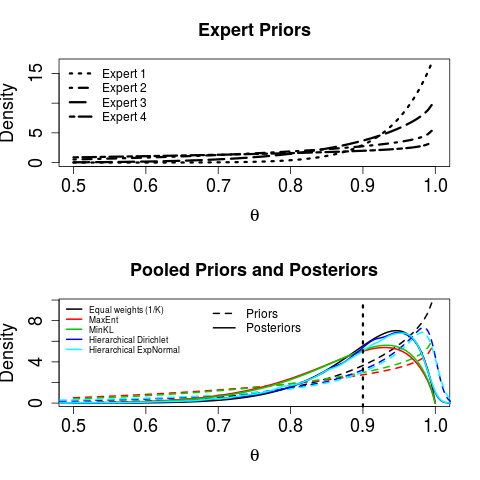
\includegraphics[width=\textwidth, height = 15cm]{figures/new_beta_example.png}
\caption{\textbf{Prior and posterior densities for $\theta$}.
Top panel shows the distributions elicited by each expert (data from~\cite{savchuk1994}) and the bottom panel shows the pooled priors and posteriors obtained using each of the three methods discussed in this paper.
The dashed vertical line marks the maximum likelihood estimate of $\theta$, $\hat{\theta}= 9/10$.
[NEEDS CHANGING]}
\label{fig:priors_posteriors_beta}
\end{figure}

\newpage

\section*{Appendix}

\subsection*{Proofs}

Here we provide a simple proof of theorem~\ref{thm:normalisation} using H\"{o}lder's inequality.
\begin{proof}
We begin by noting that $\pi(\theta)$ can be re-written as:
\begin{equation}
\label{eq:pirewritten}
 \pi(\theta) \propto f_0(\theta)\prod_{j=1}^{K} \left(\frac{f_j(\theta)}{f_0(\theta)}\right)^{\alpha_j}.
\end{equation}
Let $X_j = \frac{f_j(\theta)}{f_0(\theta)}, j=1, 2,\ldots, K$. 
Then integrating the expression in (\ref{eq:pirewritten}) is equivalent to finding 
\begin{equation}
\label{eq:expectations}
E_{0}\left[\prod_{j=1}^KX_j^{\alpha_j}\right] \leq \prod_{j=1}^KE_{0}[X_j]^{\alpha_j},
\end{equation}
where $E_{0}[\cdot]$ is the expectation w.r.t $f_0$ and (\ref{eq:expectations}) follows from H\"{o}lder's inequality for expectations~\citep{yeh2011}.
Since $\forall j$ we have $E_{0}[X_j]^{\alpha_j} = \left(\int_{\boldsymbol\Theta}f_0(\theta)\frac{f_j(\theta)}{f_0(\theta)}\right)^{\alpha_j}d\theta=1^{\alpha_j}=1$, Theorem~\ref{thm:normalisation} is proven.
\end{proof}
It is straightforward to show that remark~\ref{rmk:concavity} holds:
\begin{proof}
\begin{align}
 \pi(\theta) &\propto \prod_{i=0}^{K} [\exp(\psi_i(\theta))]^{\alpha_i}\\
             &\propto \exp(\psi^{\ast}(\theta)),
\end{align}
 where $\psi^{\ast}(\theta) = \sum_{i=0}^{K}\alpha_i\psi_i(\theta)$ is a concave function due to being a linear combination of concave functions.
\end{proof}
To see that equation~\ref{eq:entropypriorEF} holds:
\begin{eqnarray*} 
H_\pi(\theta) & = & E[-\log(\pi(\theta)] \\
              & = & - \int \log(\pi(\theta) \pi(\theta) d\theta \\
              & = & - \int (\log(K(a^*, b^*) + \theta a^* - \psi(\theta) b^*) \pi(\theta) d\theta \\
              & = & - \log(K(a^*, b^*) + a^*  E[\theta]-  b^*  E[\psi(\theta)]
\end{eqnarray*}
Likewise for equation~\ref{eq:KLpriorEF}, we have 
\begin{eqnarray*} 
KL(f_i || \pi) & = & E_\pi[\log(f_i(\theta)-\log(\pi(\theta)] \\
              & = & \int [\log( K(a_i,b_i) e^{\theta a_i - b_i \psi(\theta)}) - \log(K(a^*,b^*) e^{\theta a^* - b^* \psi(\theta)}) ] \pi(\theta) d\theta \\
              & = & \int [\log( K(a_i,b_i)) - \log(K(a^*,b^*)) + (a_i - a^*) \theta  - (b_i - b^*) \psi(\theta) \pi(\theta) d\theta \\
              & = & \log( K(a_i,b_i)) - \log(K(a^*,b^*)) + (a_i - a^*) E[\theta] - (b_i - b^*) E[\psi(\theta)] 
\end{eqnarray*}
\end{document} 